\section{Motivation}




%Overlay multicast in the cloud presents a number of new considerations, such as cloud pricing models for networking and compute resources as well as resource constraints (e.g., instance limits, per-VM egress limits) imposed by providers.

\begin{figure}[t]
     \centering
     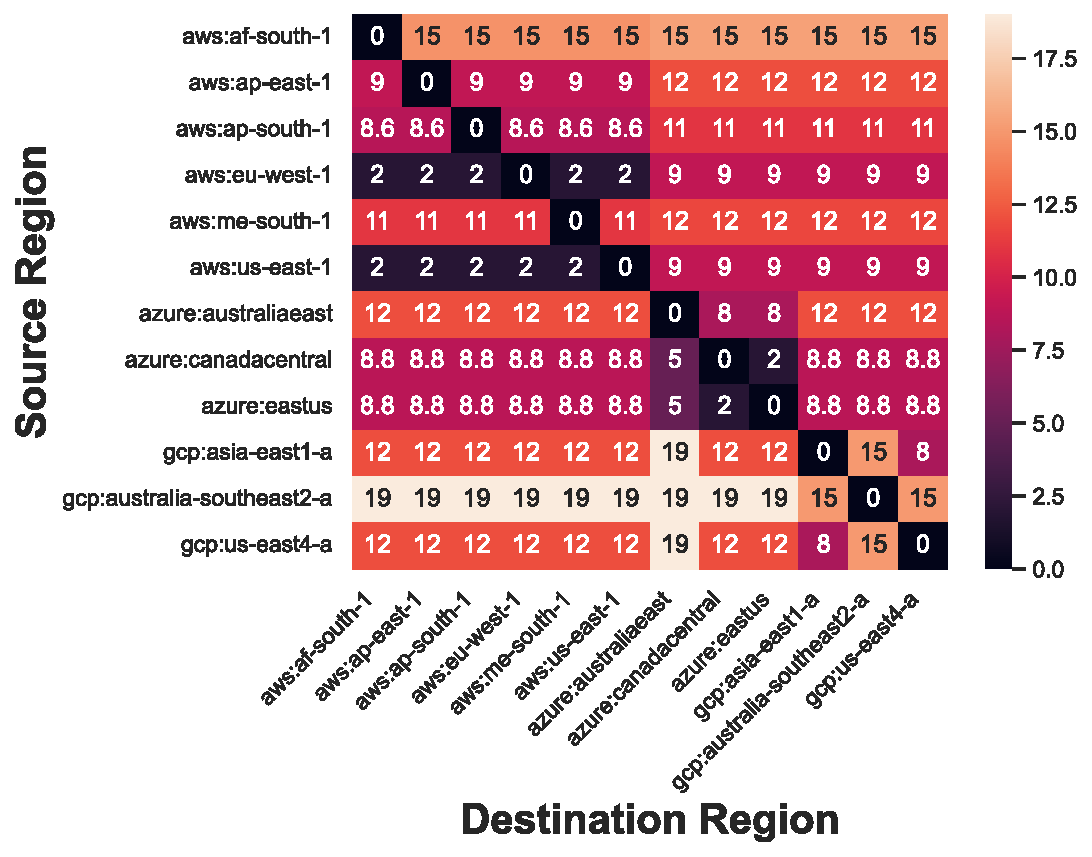
\includegraphics[width=\linewidth]{figures/cost_heatmap.pdf}
     %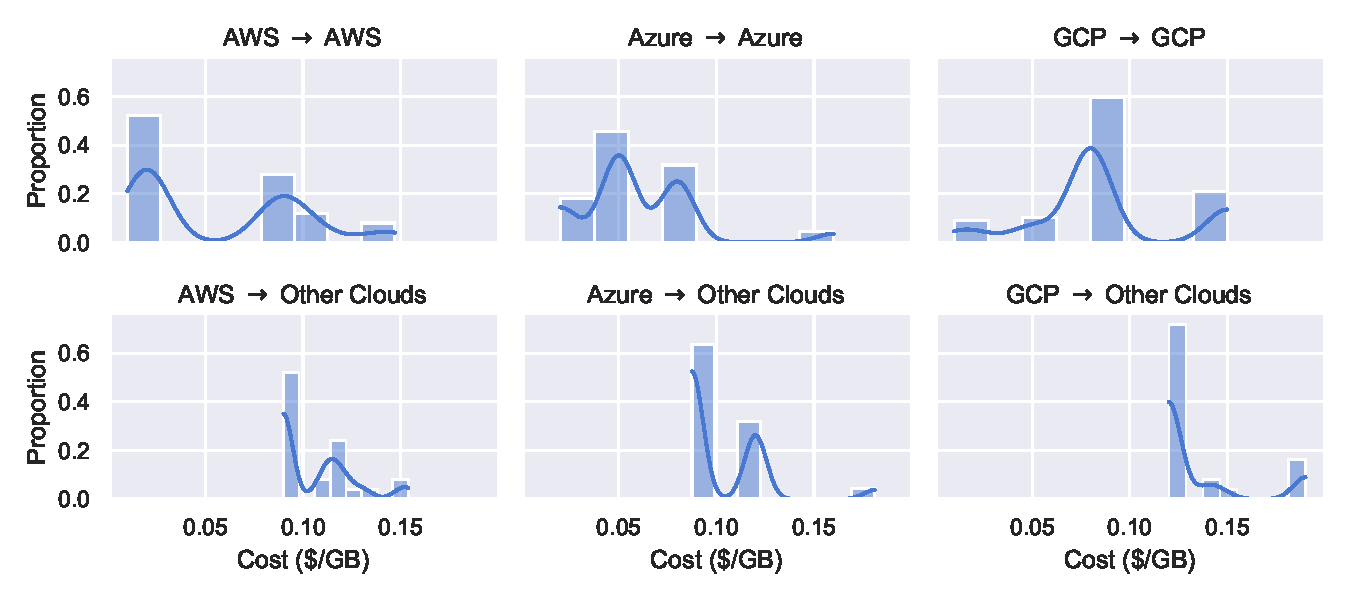
\includegraphics[width=\linewidth]{figures/2-3-cost-histograms.pdf}
     \caption{\textbf{Egress fees between regions (in cents per GB).} Egress fees are generally lower for intra-cloud transfers, but some specific regions have higher baseline egress costs. Pricing across region pairs can vary up to 19$\times$. \todo{potentially change color scheme?} \shu{lighter to represent cheaper}}
     \label{fig:cost_heatmap}
\end{figure}


%To represent the cost of overlay cloud multicast, both the prices of compute and networking resources must be incorporated into the cost. In addition to egress fees, VM instances are charged for their running duration during the transfer. However, egress fees typically dominate VM costs (up to $20\times$ for inter-cloud links).



%%%%%%%%%%%%%%%%%%%%%%%%%%%%%%%%
\subsection{Challenges of Multicast in the Cloud}
%%%%%%%%%%%%%%%%%%%%%%%%%%%%%%%%
 %Each of these considerations can vary across providers, as pricing models and resource constraints are heterogeneous~\ion{what is the difference between "heterogeneous" and "vary across providers"? Just use the same terminology.} across clouds. As a result, optimizing multicast price and replication time can be complex. 

\begin{figure*}[t!]
    \centering
    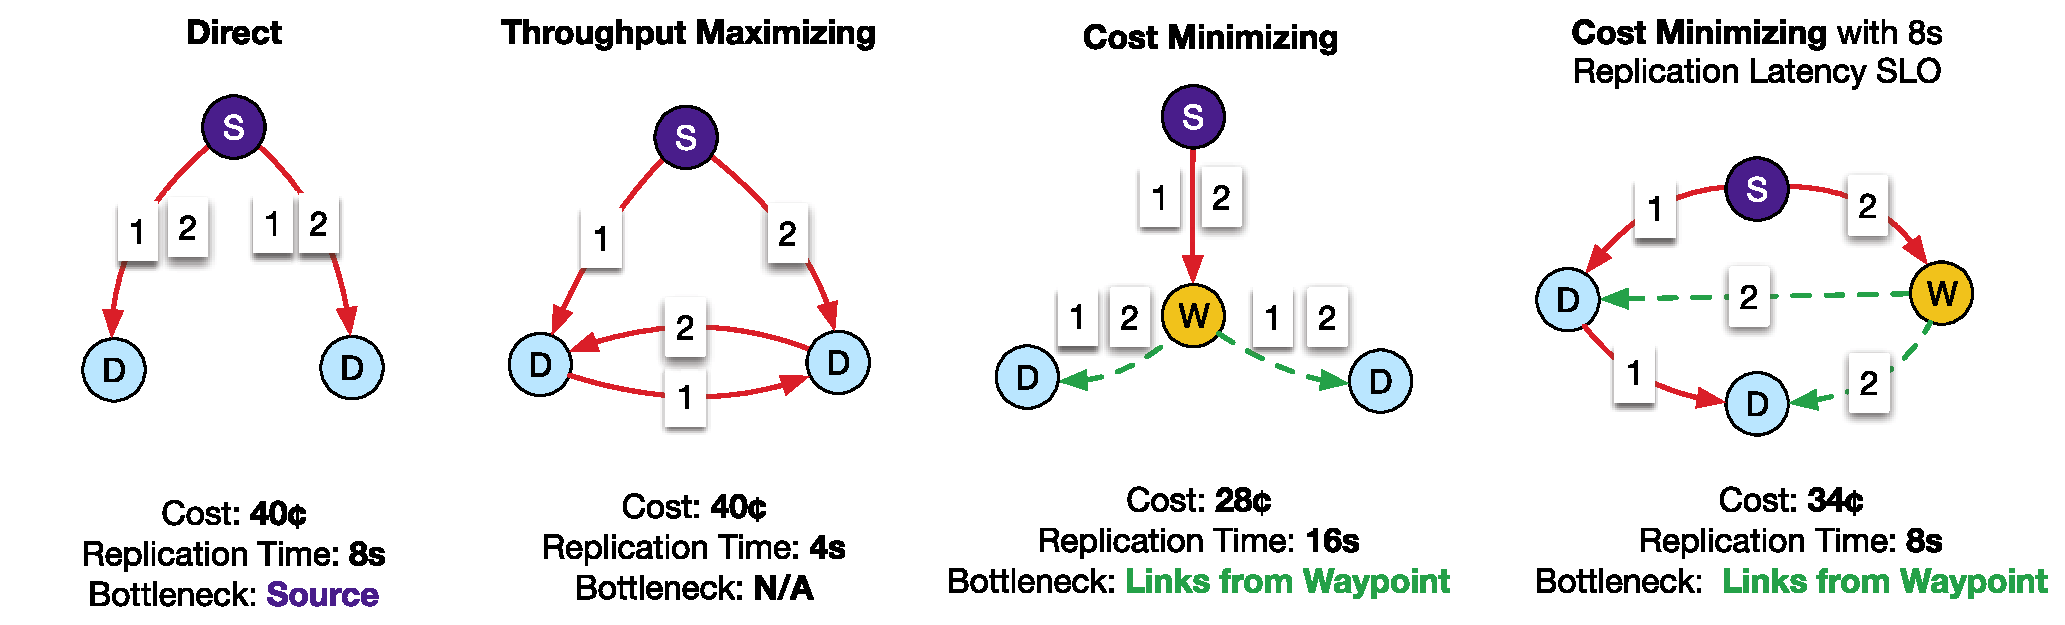
\includegraphics[width=.85\linewidth]{figures/toy_example.pdf}
    \caption{\boldmath Overlay node set and distribution trees for a toy example:  The source and destination nodes are marked `S' and `D' respectively, while waypoint nodes in yellow are marked `W'. Expensive, fast links ($\$0.1$ per GB, $2$\,Gbps) are shown in solid red, while slow, cheap links ($\$0.02$ per GB, $1$\,Gbps) are shown in dashed green. In the \textit{Direct} tree, the source node egress (4Gbps) is the bottleneck in sending out 8GB ($4 \times 2$GB stripes) of data, while both the \textit{Cost Minimizing} trees, the outgoing links from the waypoints ($1$\,Gbps) are the bottleneck. For the \textit{Throughput Maximizing} tree, all link bandwidth is used to full capacity (2Gbps) to each send $2$GB stripes, and are not bottlenecked by node egress or other links' bandwidth. 
    %\simon{This needs to be move up to earlier pages. This is a good "motivation plot".\sarah{from shu/ion:I got some feedback for the toy example 1) make it more clear on the data size (i.e. putting maybe a small graph right next to those examples showing partition 1/2 aggregate size) and 2) make it more clear on how the replication time is calculated (it’s described in the text and caption, it’s better to have text right next to the link showing what’s the bottleneck bandwidth or something similar to that; make it more intuitive on understanding why the topology is slow)}}
    } 
    \label{fig:toy_example}
\end{figure*}

% \vincent{This subsection seems to duplicate the information of the previous subsection.  I would suggest merging 2.1 and 2.2 (move the first paragraph of 2.1 into 2.0 and make 2.1 a unified "challenges" subsection).  If you really wanted to keep them separate, I think 2.2 needs to be much shorter and punchier.}


 

%At the same time, there is an opportunity in the flexibility offered by the cloud: cloud elasticity can be used to allocate a variable number of overlay nodes in specific regions to improve multicast tree performance and throughput. In this section, we describe the challenges in modeling and optimizing multicast cost. 

Cloud data replication presents several new considerations compared to traditional multicast scenarios, many stemming from the unique ways in which modern providers manage and restrict resource utilization. 

\heading{Price of multicast in the cloud}  One way in which providers manage resource utilization is through pricing.
%Cloud providers offer a variety of services, with different pricing models applied to different services.
For example, Virtual Machines (VMs) are priced based on  \textit{per second} of virtual machine usage, while networking resources are priced \textit{per unit volume} (GB) of the data transferred and depend on whether the data is crossing region or cloud boundaries.
Different cloud providers have varying pricing models, but typically networking within the same region is free, while data egress out of the cloud is charged at the highest rates. Cross-region egress (data movement within the same cloud provider) is charged somewhere in-between, with some providers (e.g., IBM, Cloudflare) offering free cross-region egress but other clouds (e.g., AWS, GCP, Azure) charging between $\$0.01-\$0.19$, depending on the source and destination region (shown in \cref{fig:cost_heatmap}). For example, GCP charges $\$0.05$ for transfers in/out of Asia regions but $\$0.02$ for US regions.


Why is it challenging to integrate pricing information into multicast?
% 
First, conventional formulations of the problem only consider allocating throughput between regions.
% 
However, egress fees in the cloud are priced according to data volume (i.e., \$ per GB) instead of throughput (i.e., \$ per Gbps).
%
Second, overlay multicast relies on the use cloud VM which are price per-second. A such, longer runtimes or the use of additional VMs (e.g. to use additional regions or improve parallism) can result in additional costs that must be co-optimized along side egress costs. 
% 
%Furthermore, cloud VM resources are also subject to per-second fees, which must be considered in selecting the number of overlay nodes created. 
\ion{What is special about "pre-second" fees? The main point here is that they charge per VM instances; I think mentioning "per-second" is a distraction.}
%\sarah{I mentioned this since its the reason why the optimization problem is hard to make linear, but maybe that's too much of a detail..}
% A naive data distribution topology may repeatedly use expensive links unnecessarily, such as when transferring from a high-egress region repeatedly to multiple other destinations instead of transferring the data once to a lower-egress region once and disseminating data to destinations from there. In addition, although cloud resource elasticity can be leveraged to create more VMs to parallelize transfer execution, the additional per-second cost of VM usage must also be modeled as part of the transfer cost.  




% \heading{Elasticity of cloud networks}\ion{This para seems to be about limits rather than elasticity. In my mind elasticity refers to the fact that I can use any number of VMs and I can place waypoints in any region. Elasticity is an opportunity. Still need to mention it because it can significantly increases the search space.}
% From the perspective of tenants, cloud networks are elastic as they can access additional capacity by provisioning more resources (VMs).
% Cloud providers allocate terabits of network links between their cloud regions~\cite{jain2013b4} and run them at high utilization.
% Providers reallocate bandwidth via traffic engineering~\cite{singh2021cost,hong2018b4} to add additional capacity and manage outages.
% Some providers place limits on the elasticity of wide-area networks with AWS and GCP limiting per-VM egress bandwidth to 5 Gbps and 7 Gbps respectively.
% To have sufficient bandwidth between regions, we can increase the number of VMs created per-region. 



\heading{Meeting replication time targets}
In practice, data transfers often have a Service Level Objective (SLO) on the desired transfer completion time.
% \ion{I think these SLOs are per latency (as mentioned earlier) rather than throughput. We need to be consistent.}
% 
It is common to replicate data to a secondary region or cloud to ensure business continuity in case of a cloud outage.
% 
AWS Replication Time Control enables users to request a transfer complete within a fixed 15-minute SLO~\cite{aws-replication-time-control}.
%
However, achieving high throughput for replication can be challenging: First, cloud providers control their network traffic to allocate certain amounts of bandwidth to paths between specific regions, limiting the per-VM throughput between regions. \sarah{there should be a better way to say this} Second, cloud providers also impose artifical limits on the network egress and ingress per-VM. For example, AWS limits cross-region egress to 5Gbps per VM, as shown in \cref{fig:tp_heatmap}. Limited VM egress bandwidth is particularly problematic for multicast, where the source node bandwidth is often a bottleneck. Since the limits are imposed per VM, the per-region limits can be increased by increasing the number of VMs per region, however the number of VMs per region is also subject to limits. 

Meeting these constraints requires selecting the right waypoint regions, number of VMs, and distribution trees for data. To do so, we must optimize both the number of VMs per-region (the overlay node set) and the distribution trees together.  \sarah{Say something about how this increases the search space?} \simon{addressed in previous paragraph, the latency target is about the constriant right?}

%Since these requirements may vary across applications, ideally users can flexibly trade off cost and throughput for cloud multicast. 

% derive the number easily: add the data partition size (make the replication time clear; the cost is clear now but not the time); show the bottleneck, and show how big the block is; assume perfectly pipeline; 

% \begin{figure*}
%      \centering
%      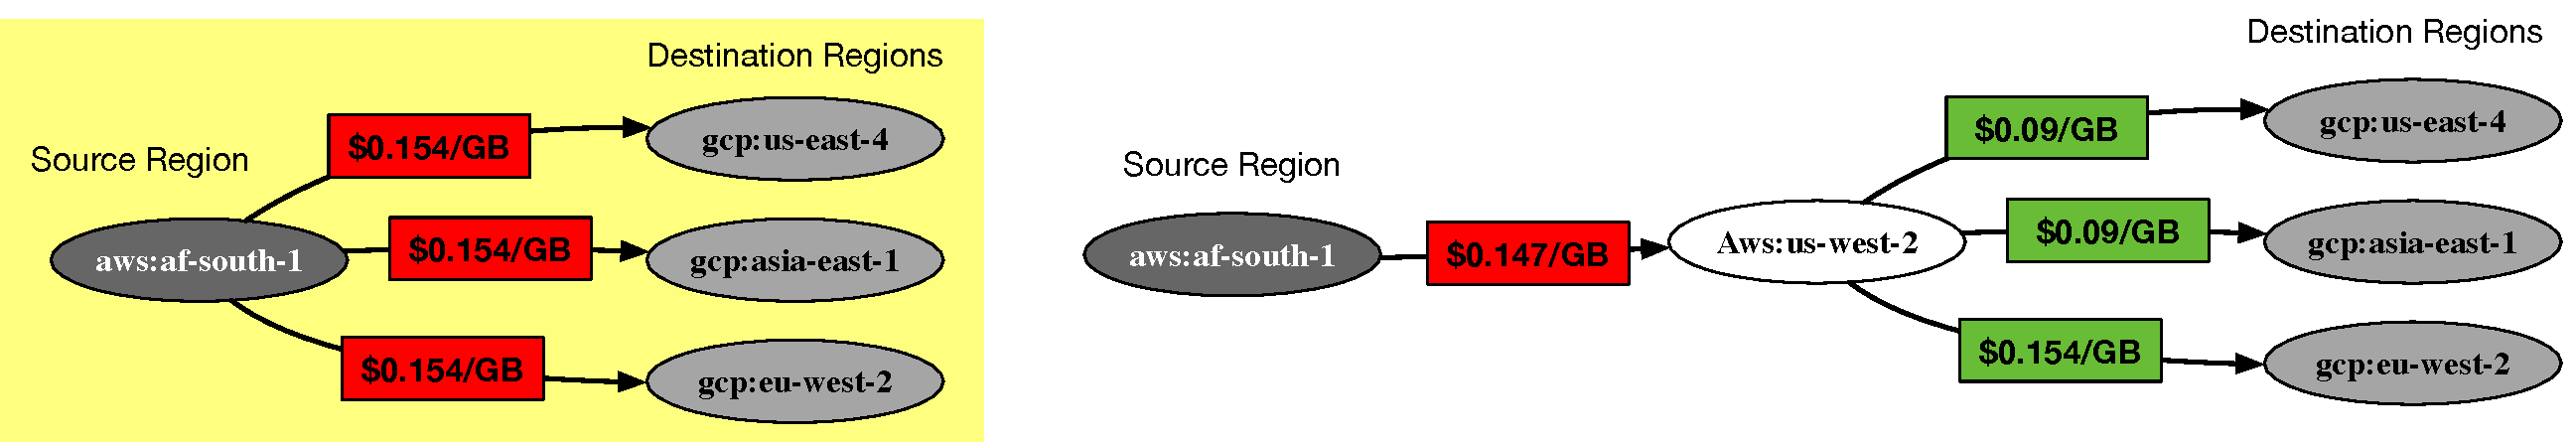
\includegraphics[width=\linewidth]{figures/overlay_example_long.pdf}
%      \caption{\textbf{Cost saving overlay region} Introducing an overlay node can reduce the overall egress cost. In the yellow box, we show a direct topology from an AWS region to three GCP regions that costs $0.462$ per GB transferred. Transferring the data to another AWS region first reduces the overall cost to $0.417$ per GB. \sarah{This is a bad example because you should just transfer to GCP once - change to AWS-only example}}
%      \label{fig:cost_overlay}
% \end{figure*}

\heading{Resource elasticity} A major advantage of the cloud is resource elasticity and the ability to flexibly create VMs across many cloud regions. While the elastic bandwidth means that we can place any number of VMs as waypoints in any regions, it significantly increased the search space for optimization: our optimizer not only controls how data is replicated across the network, but also the number of location of nodes in the network (which we refer to as the \textit{overlay node set}). 

%Cloud providers place limits on the elasticity of wide-area networks. Cloud tenants can access additional network capacity by provisioning more resources (VMs). 

%Cloud providers also impose artificial constraints on networking and compute resources. For example, AWS limits cross-region egress to 5Gbps per VM, as shown in \ref{fig:tp_heatmap}. Since the limits are imposed per VM, the per-region limits can be increased by increasing the number of VMs per region. However, additional VMs will incur additional costs, and cloud providers also limit the number of VMs that can be created per region, so per-region ingress/egress is not infinite. Limited node bandwidth is particularly problematic for multicast, where the source node bandwidth is often a bottleneck. 

%Additionally, we must account for the fact that cloud provider also caps the number of VM in each cloud, as well as pricing the compute in each region at varying rates. 



\subsection{A Simple Cloud Multicast Example}


Optimizing cost and throughput requires the selection of both the right \textit{overlay node set} as well as one or more replication trees along which data is routed. We assume data is divided into multiple \textit{stripes}, i.e. subsets of the data routed along the same replication tree, to allow for multiple concurrent replication trees. 

Consider a toy example shown in \cref{fig:toy_example} for a 2GB replication, where we have two 1GB stripes. For simplicity, we assume that all nodes have a 4Gbps bandwidth limit and we can only have one node per region. The source and destination nodes (grey) have outgoing links which are fast but expensive: each link can send at 2Gbps but costs $10\mbox{\textcent}$ per GB. However, there are other regions that have outgoing links which are cheaper but slow: they can send at 1Gbps, but cost  $2\mbox{\textcent}$ per GB. For a simple direct replication of the data from the source node to the destination nodes, the replication will be bottlenecked by the source node's egress limit (4Gbps). Because the source must send out two copies of the data, the transfer time will be 8 seconds in total. 

First, let's consider how we can optimize the throughput of the replication. We can offload egress bandwidth from the source to the destinations (an insight from \cite{castro2003splitstream}) by only sending out one copy of the data from the source. We show this in the throughput-maximizing solution, where we transfer each stripe via two different paths and peer between the destinations. 

Next, let's consider how we can also optimize the cost.  We can reduce the cost of the replication by replicating data to a waypoint region first, and then multicasting the data to the destinations from the waypoint. However, this increases our replication time by 16 seconds, which may be unacceptably slow. We can meet an 8-second replication SLO by trading off throughput for cost, by only transferring one stripe via the slower, cheaper waypoint region. 

Even for toy example, there are many different possible distribution trees, and this search space exponentially increase with more destinations, partitions, and possible waypoint regions. 

%In this toy example, we use one VM for transfer per region, and each VM has an egress limit of 4 Gbps. We show examples of possible broadcast topologies in \ref{fig:toy_example} for two stripes and two destinations. The replicated data is transferred via two stripes, represented in red and blue. A throughput-maximizing topology \textit{peers} stripes of the data to offload bandwidth from the source. The cost-minimizing solution uses an overlay region with cheaper, but slower connections to the destination regions. A cost-minimizing solution with a replication latency SLO may route part of the data through the overlay, and part of the data directly to the destinations to balance both cost and throughput. 


%\heading{What does it cost?}
%\shu{Rethinking multicast in the cloud, explain more precisely what's happening with cost and edge capacity}

%\heading{Utilizing edge capacity} Utilizing the edge capacity can be challenging due to limited node egress bandwidth. 